% !TEX root = ./informe.tex
\section{Experimentación general}

Dado que nuestros análisis estaban enfocados a los peores casos, es momento de considerar cómo son nuestras soluciones si consideramos casos promedios.  \\

Consideramos que un grafo de $n$ nodos es promedio cuando generamos sus aristas al azar. Esto significa que las conexiones entre nodos será aleatoria, pero la cantidad de aristas estará predeterminada con algun porcentaje, para poder separar mejor los diferentes casos de análisis. En particular, mostraremos los casos donde hay 50\% y 75\% de aristas. Demás porcentajes resultaron muy poco interesantes por tener muy pocas aristas o demasiadas. Como última aclaración, para todas las instancias de búsqueda local, la cantidad de repeticiones usadas es $2000$ a menos que se mencione explícitamente. \\

Nuestra intención es comparar exactamente que tan mejores o peores son los diferentes algoritmos utilizados. Para esto, para cada tamaño de $n$ generamos un grafo al azar (con cierto porcentaje de aristas) y comparamos las soluciones obtenidas por todas las técnicas. Lo que sigue no son promedios, sino las soluciones finales para algun algoritmo aleatorio dado. \\

{\centering
    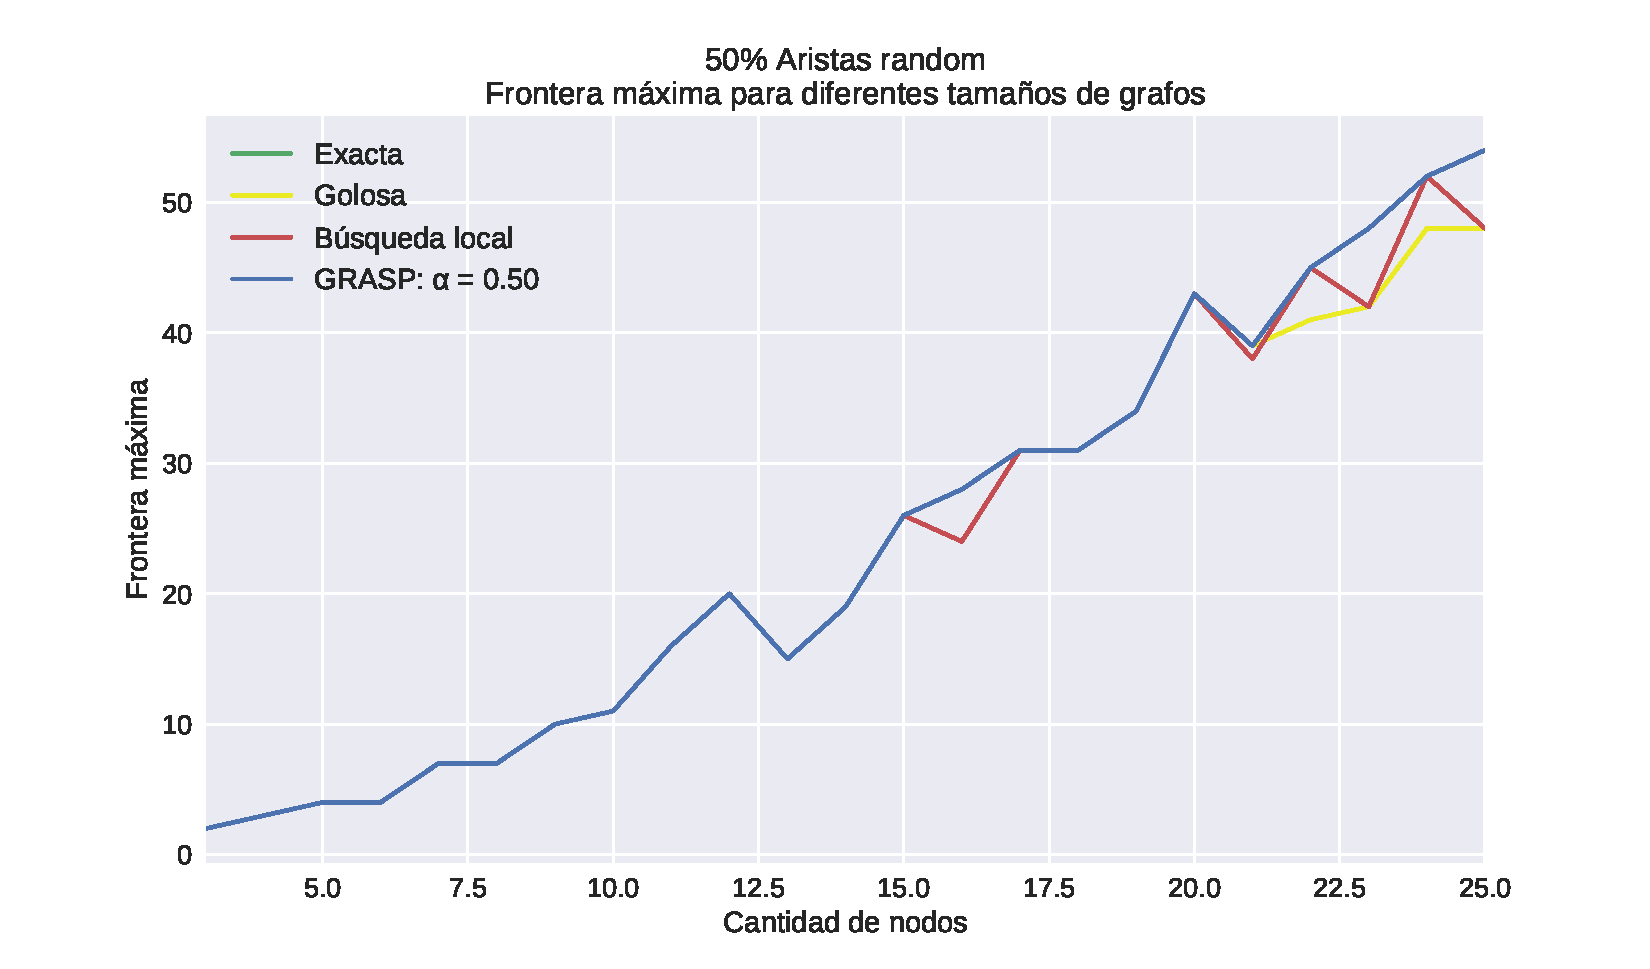
\includegraphics[width=1\textwidth]{informe/imgs/exp_random50_frontera_todos_v2.pdf}
    \captionof{figure}{$\uparrow$ Exacta y GRASP comparten la misma curva}
}
$ $ \newline

Los resultados son lo que nuestros análisis anteriores apuntaban. Debemos tener en cuenta que son valores de $n$ pequeños (para poder comparar con el algoritmo exacto), veremos más adelante comparaciones para $n$ mayores. \\

Observamos que Grasp es la mejor técnica de las presentadas para resolver el problema, de hecho comparte la misma curva que el algortimo exacto. Le siguen el algoritmo de búsqueda local, y por último el goloso. Como prometimos, si bien en el análisis para un ``grafo malo'' el greedy era extremadamente malo, aquí podemos notar que para grafos en general conseguimos una aproximación bastante buena. \\

Analicemos tambíen que pasa con los tiempos de cómputo. Como era esperable, el tiempo del algoritmo exacto crece muy rápidamente, así que mostramos el gráfico en \textit{escala logarítmica}. En general son tiempos esperados, pero es interesante notar que Grasp tiene una constante asociada mucho mas elevada que los demás. \\

{\centering
    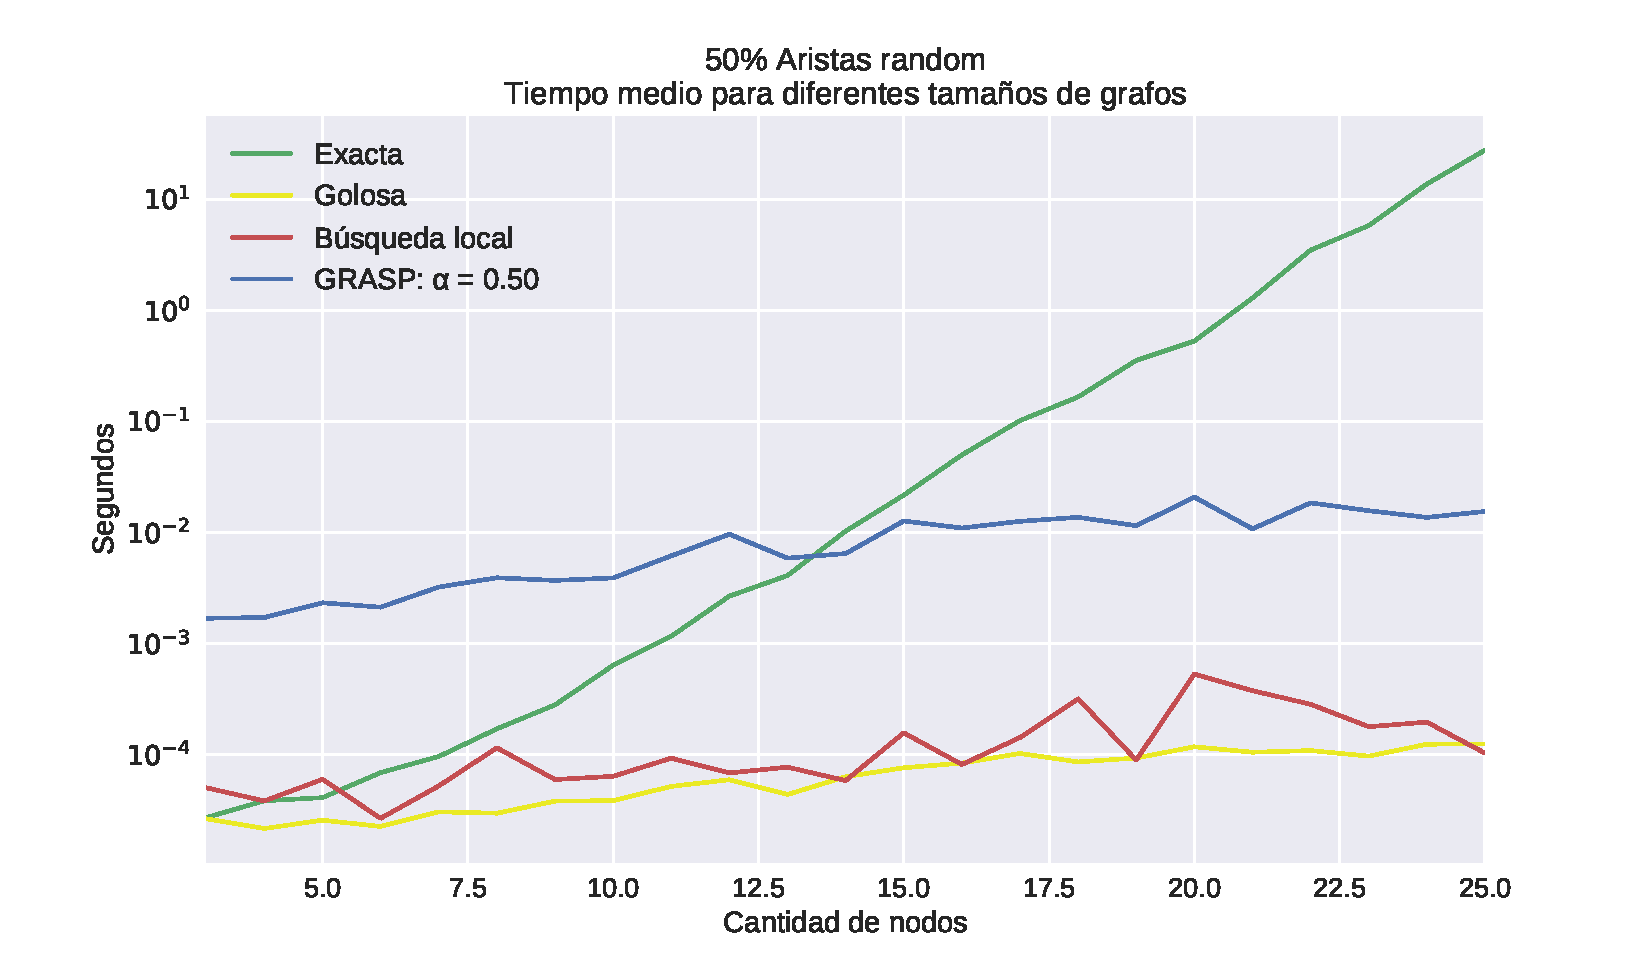
\includegraphics[width=1\textwidth]{informe/imgs/exp_random50_tiempo_todos_v2.pdf}
    \captionof{figure}{$\uparrow$ Escala logarítmica}
}
$ $ \newline

Repetimos el experimento pero para grafos con 75\% de aristas, sin embargo en todos los algoritmos nos dan la misma solución (la óptima!). Esto tiene que ver con la densidad del grafo, y probablemente porque estamos viendo tamaños pequeños. \\

{\centering
    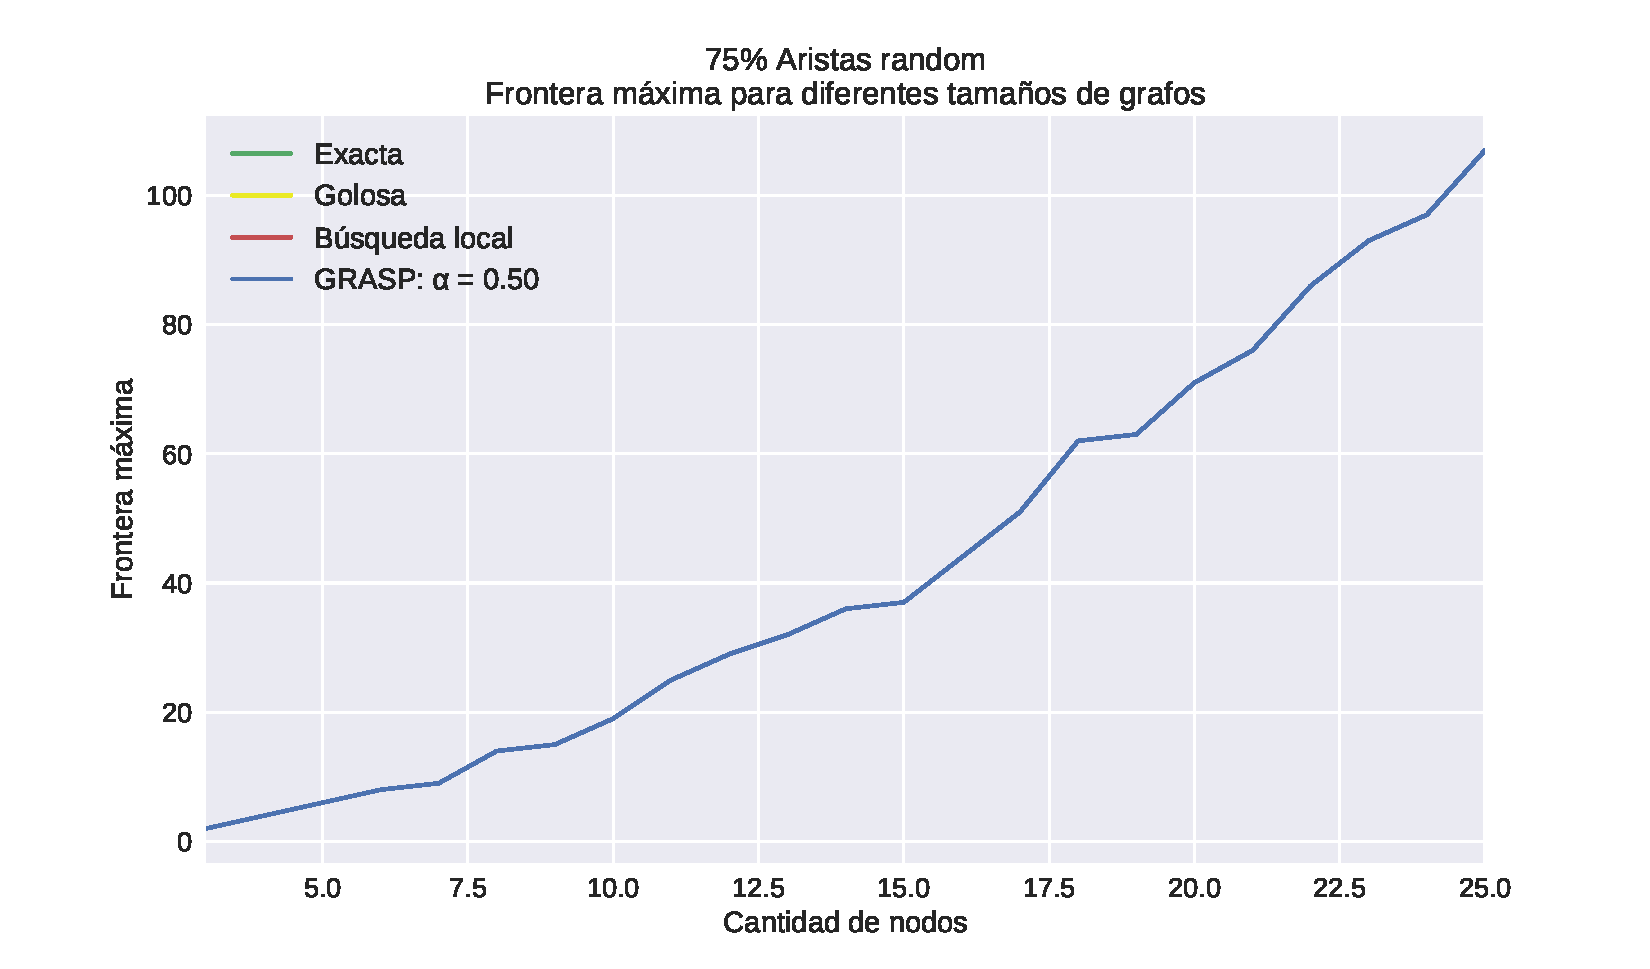
\includegraphics[width=1\textwidth]{informe/imgs/exp_random75_frontera_todos_v2.pdf}
}
$ $ \newline

Veamos que sucede si hacemos crecer $n$. Dado que no podemos realizar las pruebas para el algortimo exacto debido a su complejidad temporal, no lo incluimos en el gráfico. No vamos a tener ninguna certeza de cuán cerca o lejos están de la solución óptima, sin embargo es interesante observar como varían las diferentes soluciones. No incluímos 75\% aristas pues es idéntico al de 50\%.

{\centering
    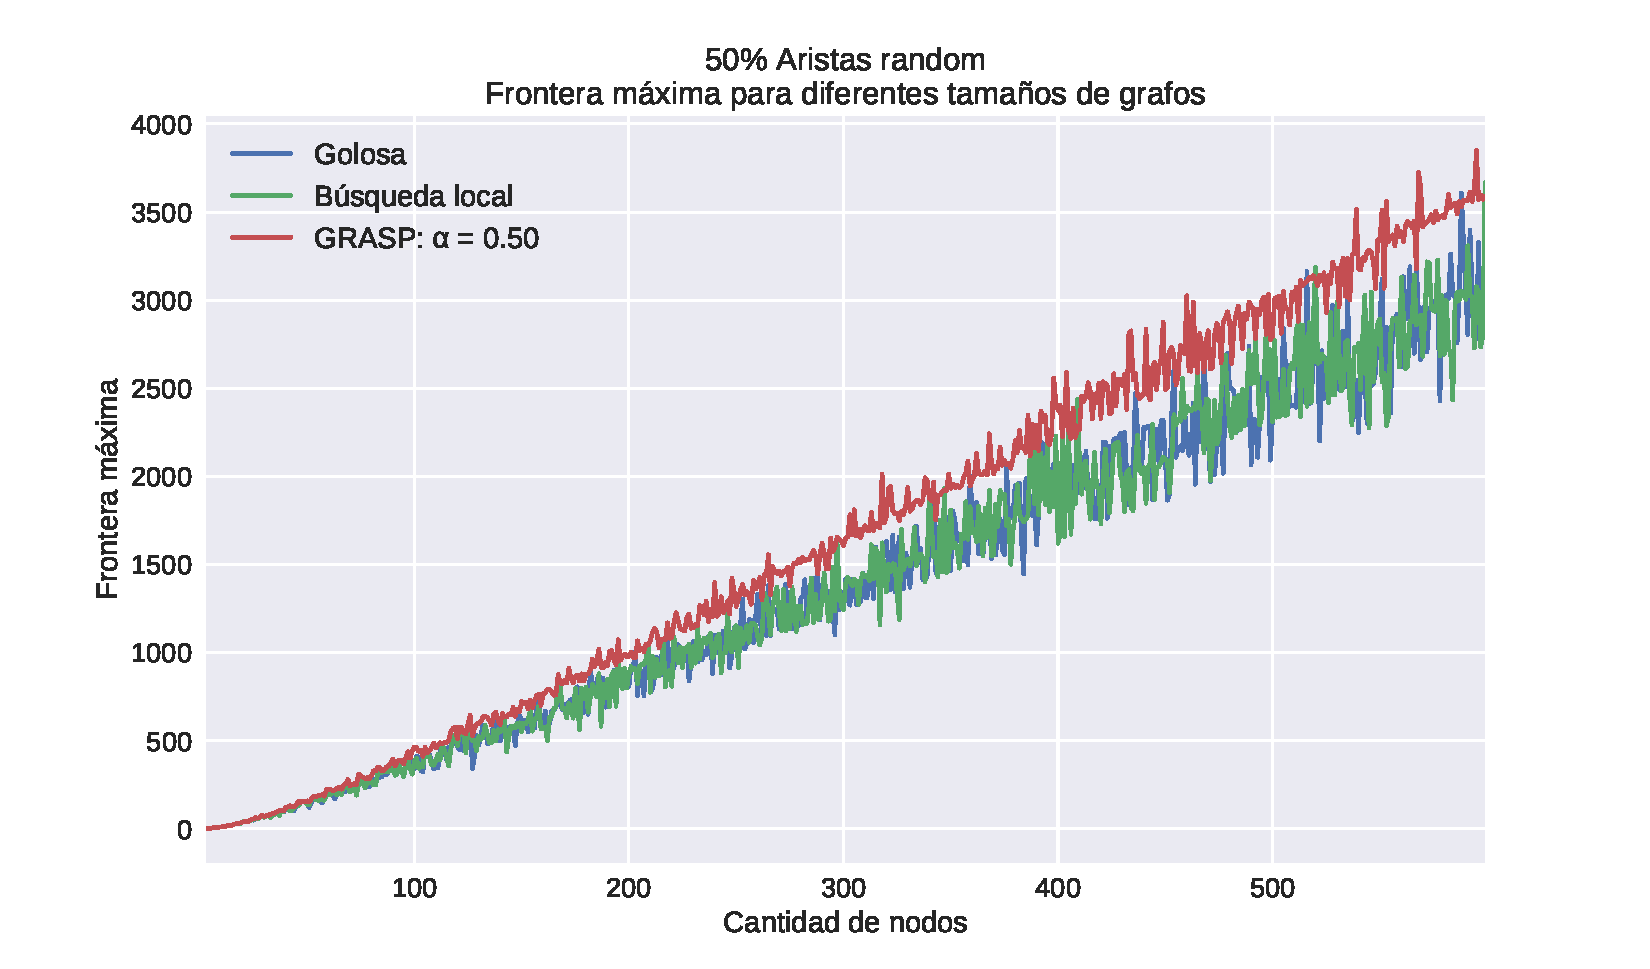
\includegraphics[width=0.9\textwidth]{informe/imgs/exp_random50_frontera_todos_ngrande.pdf}
}

Como esperábamos, Grasp es la mejor alternativa que tenemos para resolver el problema de CMF. El componente random sumado a la cantidad de repeticiones hacen que sea superior a los demás algortimos, en términos de aproximación a la solución óptima. Variando la cantidad de $repsGrasp$ no obtuvimos diferencias significativas. En el gráfico se muestra con $repsGrasp = 50$. \\

Grasp es mejor, ¿pero a qué costo? Mostramos el gráfico en \textit{escala logárítmica} debido al tamaño de los tiempos de Grasp en comparación a los demás. Podemos observar claramente que el costo temporal es incluso mayor al esperado (y quizá hasta mayor al deseado) dónde para $n = 600$ se demora aproximadamente 3 segundos.

{\centering
    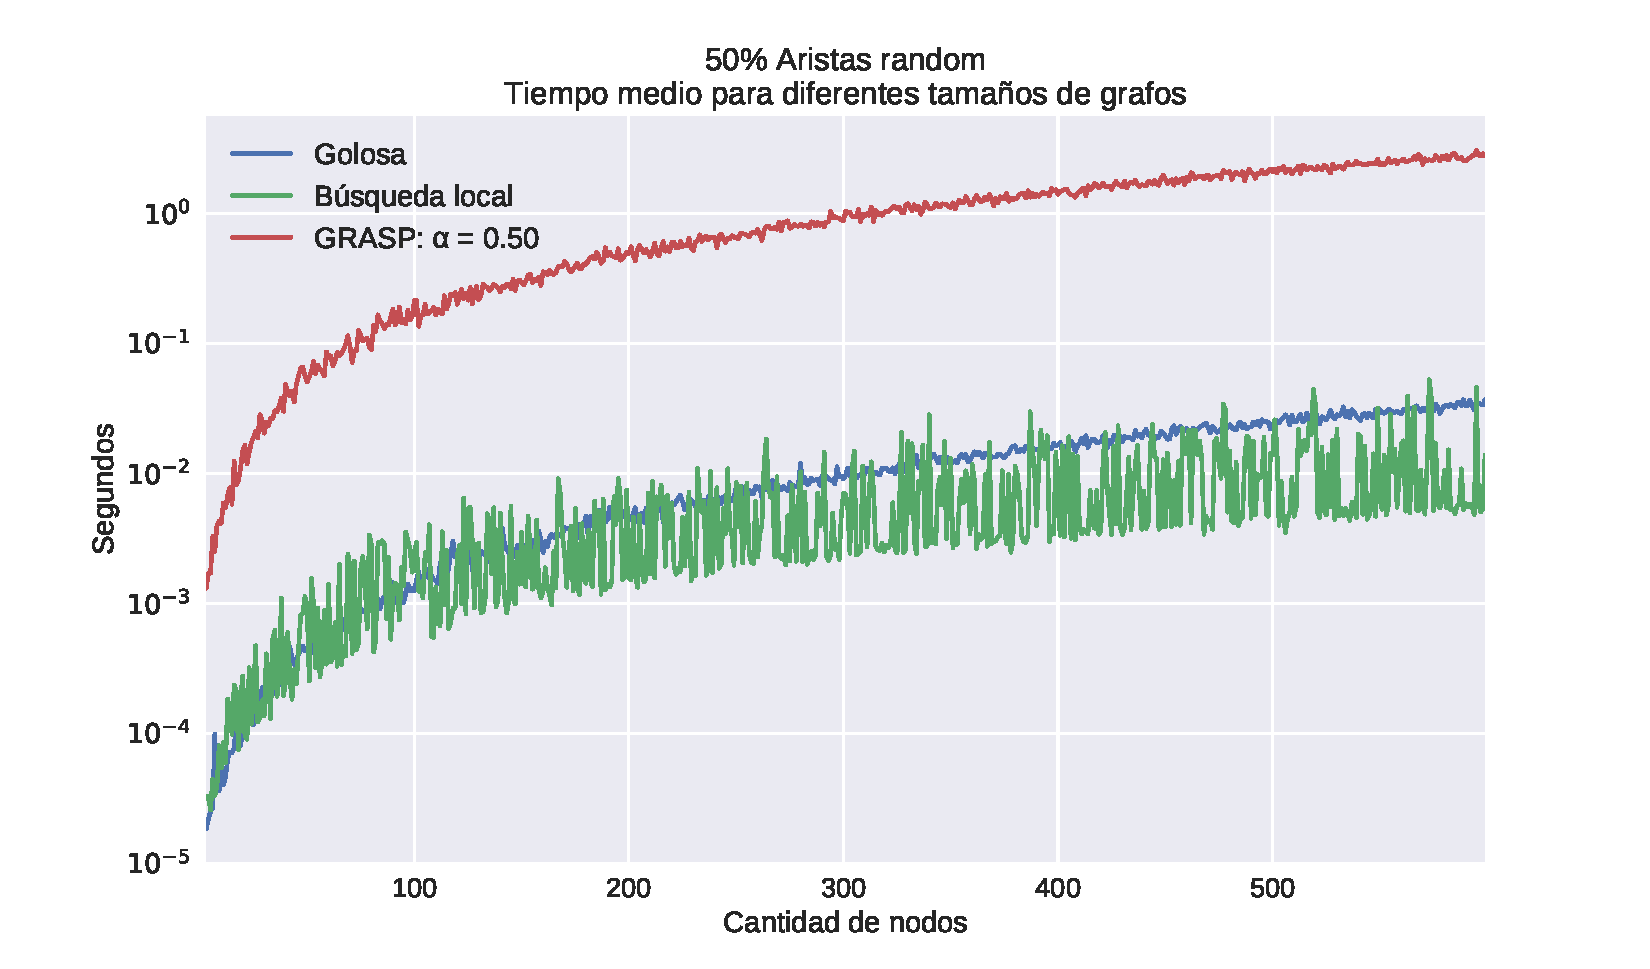
\includegraphics[width=0.9\textwidth]{informe/imgs/exp_random50_tiempo_todos_ngrande_logy.pdf}
}

El caso de tiempos de 75\% aristas no lo mostramos por ser idéntico en forma al anterior, pero en ese caso con $n = 600$ Grasp tarda aproximadamente 17 segundos. Pueden disminuirse la cantidad de iteraciones para obtener una mayor eficiencia en términos del tiempo, pero a medida que $n$ crece Grasp es el primero que se vuelve inutilizable.

% No vale la pena por ser igual a 50%
% {\centering
%     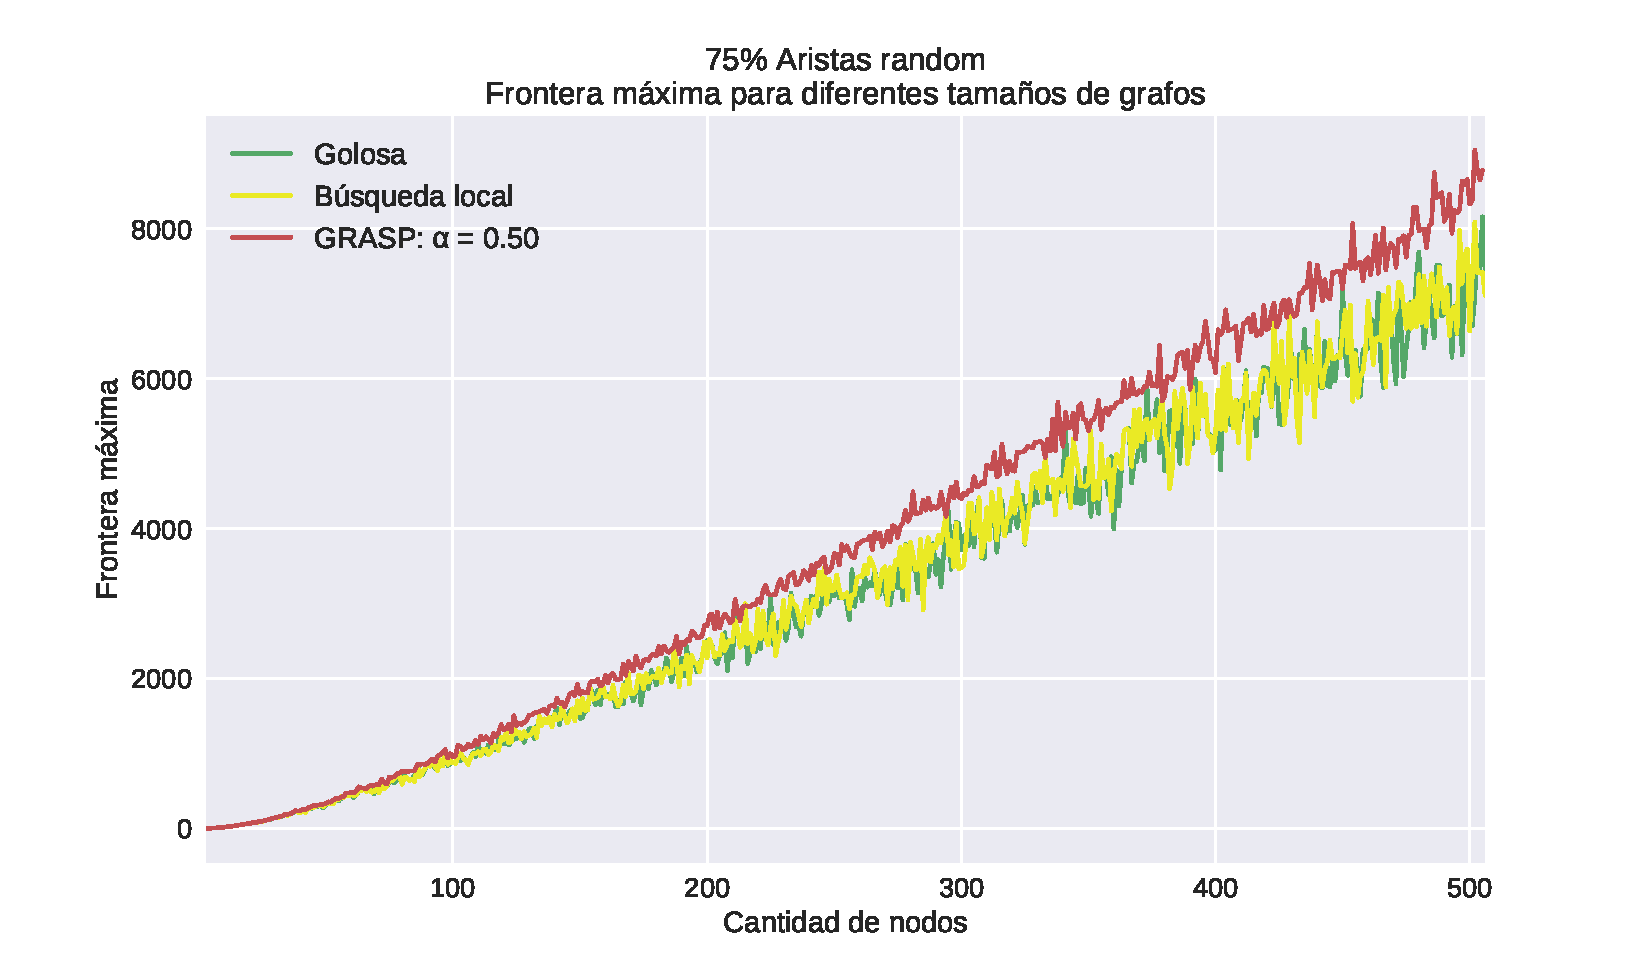
\includegraphics[width=1\textwidth]{informe/imgs/exp_random75_frontera_todos_ngrande.pdf}
% }


\subsection{Conclusión}

\todo[inline]{Cual era nuestro problema}
\todo[inline]{Por que no podemos obtener una solucion exacta}
\todo[inline]{Cuales fueron nuestras estrategias para aproximar una solucion}
\todo[inline]{Cual es la mejor estrategia}

